\chapter{जीन और DNA}\label{ch:g9:genes-and-dna}

\omterm{def:g9:chromosomes:chromosomes}{गुणसूत्र} निर्धारक ढोते हैं --- पर कोई धागा अभी कोई इबारत नहीं है। किसी
\omterm{def:g9:chromosomes:chromosomes}{गुणसूत्र} के साथ-साथ एक निर्धारक \emph{है} क्या? और वह धागा बना किस चीज़
से है, कि मिलीमीटर के हज़ारवें हिस्सों भर चौड़ा कोई \omterm{def:g6:cell-unit-of-life:parts}{केंद्रक} पूरे इंसान के
निर्देश थामे रह सके (\cref{exo:g9:heredity-and-traits:12})? इसका जवाब
दो नाम देते हैं, और वे आधुनिक जीव विज्ञान के सबसे मशहूर नाम हैं: \omterm{def:g9:genes-and-dna:gene}{जीन}, और
\omterm{def:g9:genes-and-dna:dna}{DNA}।

\section{जीन: निर्धारक, अपनी जगह पर}

\begin{definition}[जीन और विकल्पी]\label{def:g9:genes-and-dna:gene}
\emph{जीन}\index{जीन} एक निर्धारक का ठीक-ठीक रूप है: यानी किसी
\emph{\omterm{def:g9:chromosomes:chromosomes}{गुणसूत्र} का एक टुकड़ा}, जो किसी एक \omterm{def:g9:heredity-and-traits:traits}{लक्षण} की बनावट के हिस्से के
निर्देश ढोता है --- एक जीन रक्त-समूह की मशीनरी के लिए, दूसरे \omterm{def:g1:the-five-senses:sense}{आँखों} के
रंग के वर्णकों के लिए, और उन 46 धागों पर हज़ारों-हज़ार, हर एक अपने तय पते
पर। कोई जीन कई रूपों में मौजूद हो सकता है --- यानी
\emph{विकल्पी}\index{विकल्पी}: रक्त-समूह वाले जीन के A, B और O रूप, और
\omterm{def:g1:the-five-senses:sense}{आँखों} के रंग वाले जीन के भूरा और नीला। पता वही, हिज्जे अलग।
\end{definition}

\begin{proposition}[दो प्रतियाँ, और दिखने का मतलब]\label{prop:g9:genes-and-dna:twocopies}
\omterm{def:g9:chromosomes:chromosomes}{गुणसूत्र} जोड़ों में आते हैं (\cref{prop:g9:chromosomes:counts}) ---
इसलिए हर \omterm{def:g9:genes-and-dna:gene}{जीन} \emph{दो प्रतियों} में आता है, हर साथी पर एक, और हर जनक से
एक। वे दोनों प्रतियाँ एक ही \omterm{def:g9:genes-and-dna:gene}{विकल्पी} हो सकती हैं या अलग-अलग; और अलग हों तो
हो सकता है कि एक \emph{व्यक्त} हो और दूसरी चुपचाप ढोई जाए --- और इसी के
साथ परिवार के एलबम के रहस्य कार्य-प्रणाली में बदल जाते हैं:
\begin{itemize}
  \item बिना दिखे ढोना (\cref{ex:g9:heredity-and-traits:skip}): वह
        चुप \omterm{def:g9:genes-and-dna:gene}{विकल्पी} दूसरे साथी पर सवार होती है;
  \item A और B वाले जनकों की O समूह वाली संतान
        (\cref{pb:g9:heredity-and-traits:1}): हर जनक ने O चुपचाप ढोया
        था, और आधा करने ने दोनों O एक साथ बाँट दिए;
  \item भूरी \omterm{def:g1:the-five-senses:sense}{आँखों} वाले जनकों की नीली \omterm{def:g1:the-five-senses:sense}{आँखों} वाली संतान: दो चुप नीली
        \omterm{def:g9:genes-and-dna:gene}{विकल्पियों} का मिलना --- और यह चार में एक मौक़ा है, जब दोनों जनक
        एक-एक ढोते हों: आधा करना हर जनक की नीली को दो में एक मौक़े से
        बाँटता है, और दोनों बँटवारे एक-दूसरे से आज़ाद हैं।
\end{itemize}
\end{proposition}
\admitted

\begin{example}[रक्त-समूह, पूरी तरह मशीन में उतरे हुए]\label{ex:g9:genes-and-dna:bloodgroups}
एक \omterm{def:g9:genes-and-dna:gene}{जीन}, तीन \omterm{def:g9:genes-and-dna:gene}{विकल्पी}, और हर व्यक्ति में दो प्रतियाँ: A के साथ A या O हो
तो समूह A दिखता है; B के साथ B या O हो तो B; A के साथ B हो तो AB (दोनों
व्यक्त --- यानी \omterm{def:g9:genes-and-dna:gene}{विकल्पियों} को हमेशा चुप नहीं किया जा सकता); और O के साथ
O हो तो O। रक्तदान की बही का पूरा ढर्रा --- और उसका हर ``चौंकाने वाला''
मामला भी --- दो प्रतियों वाले बँटवारों का गणित ही है।
\end{example}

\section{DNA: यह इबारत लिखी किस चीज़ में है}

\begin{definition}[DNA]\label{def:g9:genes-and-dna:dna}
रसायन के लिहाज़ से कोई \omterm{def:g9:chromosomes:chromosomes}{गुणसूत्र} \emph{DNA}\index{DNA} का एक बेहद लंबा,
लिपटा हुआ अणु है (और साथ में उसे बाँधने वाले प्रोटीन): यानी एक दोहरी लड़ी
--- वही मशहूर ऐंठी हुई सीढ़ी --- जिसके डंडे चार रासायनिक अक्षरों के जोड़े
हैं। \emph{लड़ी के साथ-साथ उन अक्षरों का क्रम ही जानकारी है}: कोई \omterm{def:g9:genes-and-dna:gene}{जीन} उसी
अनुक्रम का एक हिस्सा है, जैसे कोई वाक्य किसी पन्ने का हिस्सा होता है। चार
अक्षर, और इंसान की एक गड्डी में उनके तीन अरब --- यानी किसी पूरी बनावट के
निर्देशों भर की इबारत, हर \omterm{def:g6:cell-unit-of-life:parts}{केंद्रक} में लिपटी हुई।
\end{definition}

\begin{example}[उसे ख़ुद देखना]\label{ex:g9:genes-and-dna:extraction}
\omterm{def:g9:genes-and-dna:dna}{DNA} रसोई में ही निकाला जा सकता है: किसी केले या प्याज़ को मसलो, उसमें
नमकीन पानी और थोड़ा बरतन धोने वाला तरल मिलाओ (\omterm{def:g6:cell-unit-of-life:parts}{झिल्लियाँ} खोल दी गईं ---
\cref{def:g6:cell-unit-of-life:parts} वाले लिफ़ाफ़े ही उसका निशाना हैं),
छानो, और ऊपर से ठंडी स्पिरिट की एक परत डालो: दोनों की सरहद पर सफ़ेदी
लिए धागों का एक गुच्छा उठ आता है, जिसे किसी तिनके पर लपेटा जा सकता है। वे
धागे \omterm{def:g9:genes-and-dna:dna}{DNA} हैं --- यानी इस अध्याय का असली अणु, असली सेंटीमीटरों में।
\end{example}

\begin{omfigure}
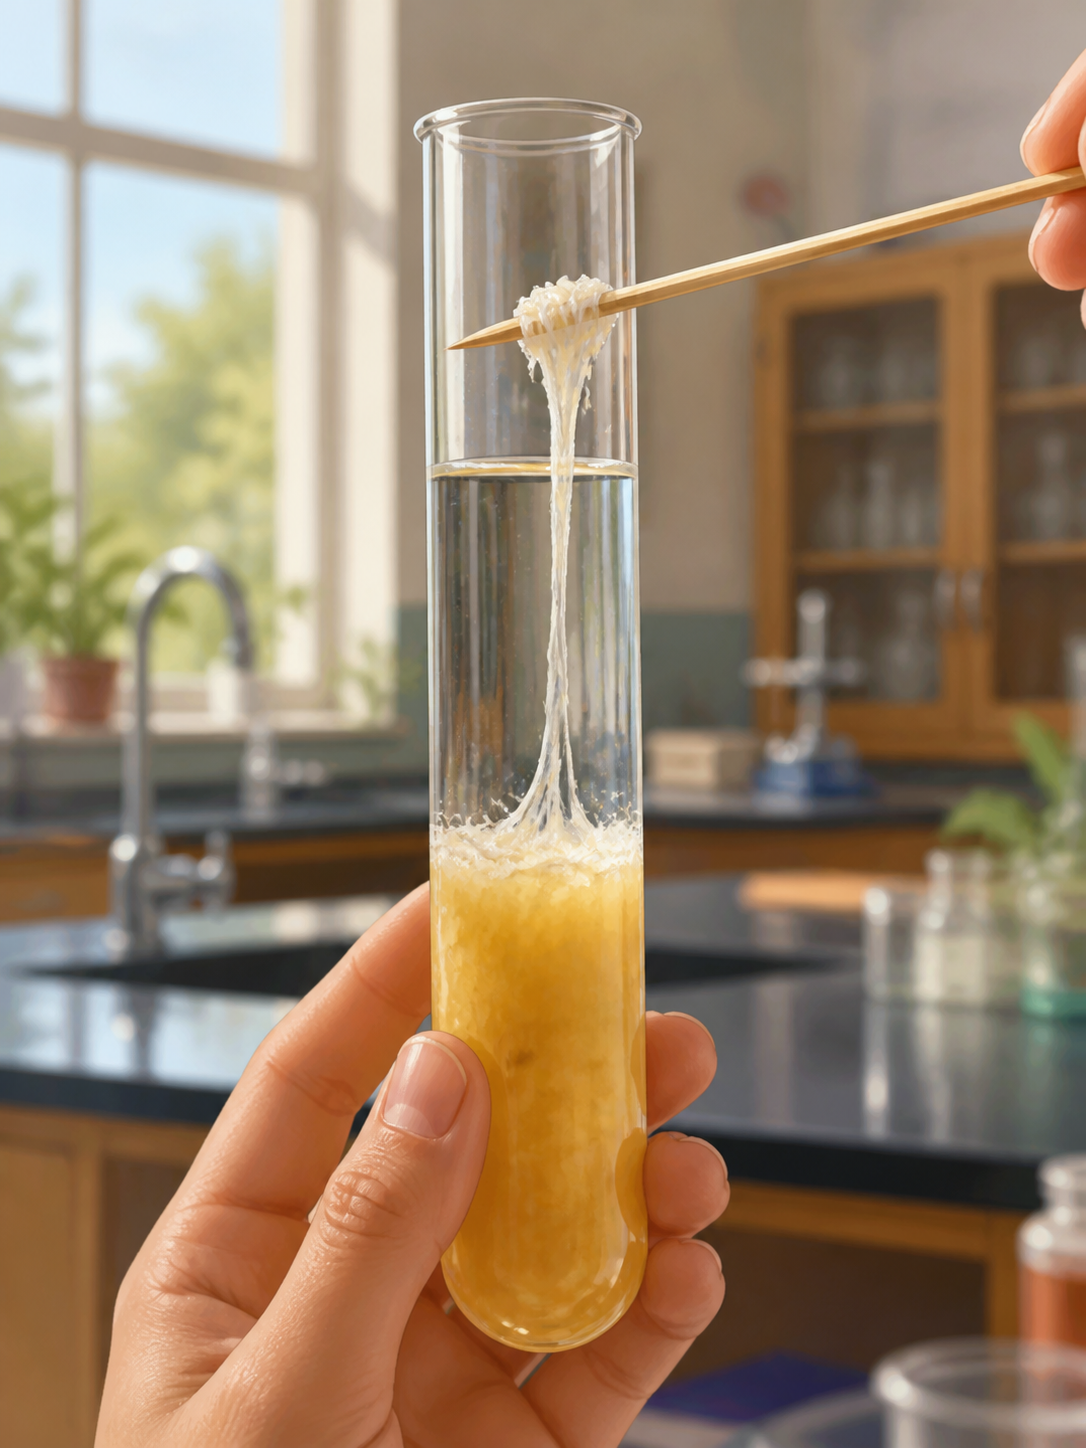
\includegraphics[width=0.42\linewidth]{images/book1/ai/g9-dna-extraction.png}

{\small रसोई वाले निकालने का इनाम: \omterm{def:g9:heredity-and-traits:heredity}{आनुवंशिकता} का अणु, एक तिनके पर लपेटा
हुआ।}
\end{omfigure}

\begin{proposition}[DNA की बनावट क्या-क्या समझाती है]\label{prop:g9:genes-and-dna:explains}
वह दोहरी लड़ी कोई सजावट नहीं --- उसका हर गुण किसी पुराने सवाल का जवाब
देता है:
\begin{itemize}
  \item \emph{नक़ल}
        (\cref{prop:g5:first-look-at-cells:growth} वाले वफ़ादार
        बँटवारे): दोनों लड़ियाँ अक्षर-दर-अक्षर एक-दूसरे की पूरक हैं,
        इसलिए अलग खींची जाएँ तो हर एक अपना साथी दोबारा बना लेती है ---
        यानी एक सीढ़ी से दो एक-सी सीढ़ियाँ, हर बेटी-कोशिका के लिए एक;
  \item \emph{\omterm{def:g9:genes-and-dna:gene}{विकल्पी}}: किसी \omterm{def:g9:genes-and-dna:gene}{जीन} के रूप उस अनुक्रम में हिज्जों के
        छोटे-छोटे फ़र्क़ हैं --- वही पता, बदले हुए अक्षर;
  \item \emph{उत्परिवर्तन}\index{उत्परिवर्तन}: नक़ल लगभग मुकम्मल है,
        मुकम्मल नहीं --- कभी-कभार ग़लत उतरा एक अक्षर एक \emph{नई}
        \omterm{def:g9:genes-and-dna:gene}{विकल्पी} बना देता है। ज़्यादातर बेअसर, कभी नुक़सानदेह, और
        कभी-कभार उपयोगी: \omterm{prop:g9:genes-and-dna:explains}{उत्परिवर्तन} ही वह जगह है जहाँ से नए हिज्जे,
        और आख़िरकार सारी \omterm{def:g9:genes-and-dna:gene}{विकल्पियाँ}, आती हैं --- यानी वही कच्चा
        नयापन, जो \cref{ch:g9:how-species-change} को चाहिए होगा;
  \item \emph{पढ़ना}: कोई \omterm{def:g5:first-look-at-cells:cell}{कोशिका} किसी \omterm{def:g9:genes-and-dna:gene}{जीन} का इस्तेमाल उसका अनुक्रम
        पढ़कर और उससे मेल खाता काम करने वाला अणु बनाकर करती है ---
        और हर तरह की \omterm{def:g5:first-look-at-cells:cell}{कोशिका} उस पुस्तकालय में से अपना ही चुनाव पढ़ती
        है: यानी \cref{exo:g9:chromosomes:12} वाली पहेली, जैसा वादा
        था वैसे ही हल हुई।
\end{itemize}
\end{proposition}
\admitted

\begin{remark}[एक ही कूट, और पूरा जीवन]\label{rem:g9:genes-and-dna:universal}
सबसे गहरा तथ्य सबसे आख़िर में आता है: \emph{हर} \omterm{def:g6:exploring-our-environment:components}{सजीव} अपने \omterm{def:g9:genes-and-dna:gene}{जीन} उन्हीं \omterm{def:g9:genes-and-dna:dna}{DNA}
अक्षरों में लिखता है और उन्हें उसी कूट से पढ़ता है --- बलूत, ख़मीर,
ह्वेल, \cref{ch:g6:producing-our-food} वाले सूक्ष्मजीव, और तुम भी। यही
\omterm{prop:g5:first-look-at-cells:principle}{जीवन की एकता} (\cref{prop:g5:first-look-at-cells:principle}) है, अपनी नींव
पर; और \omterm{def:g6:classification-kinship:tree}{नातेदारी-वृक्ष} (\cref{rem:g6:classification-kinship:implies}) का
अब तक का सबसे मज़बूत सबूत भी: एक साझी भाषा एक साझी शुरुआत की दलील देती
है। और आनुवंशिक अभियांत्रिकी काम ही इसलिए करती है --- क्योंकि \omterm{def:g5:biodiversity:species}{प्रजातियों}
के बीच ले जाया गया कोई \omterm{def:g9:genes-and-dna:gene}{जीन} तब भी पढ़ा जा सकता है, जैसे कोई वाक्य किसी और
किताब में उतार लिया गया हो।
\end{remark}

\begin{method}[तीन दर्जों की पढ़त]\label{met:g9:genes-and-dna:levels}
\omterm{def:g9:heredity-and-traits:heredity}{आनुवंशिकता} का कोई भी सवाल अब तीन दर्जों पर पढ़ा जा सकता है --- और इनके
बीच बदलने की प्रैक्टिस करो:
\begin{enumerate}
  \item \emph{परिवार का दर्जा}: कौन दिखाता है, कौन ढोता है, कौन
        पहुँचाता है (\cref{ch:g9:heredity-and-traits});
  \item \emph{\omterm{def:g9:chromosomes:chromosomes}{गुणसूत्र} का दर्जा}: कौन-से धागे, आधे होकर और बहाल होकर,
        वह बँटवारा ढोते हैं (\cref{ch:g9:chromosomes});
  \item \emph{अणु का दर्जा}: कौन-सा \omterm{def:g9:genes-and-dna:gene}{जीन}, कौन-सी \omterm{def:g9:genes-and-dna:gene}{विकल्पी}, कौन-से
        हिज्जे --- और किसी नए \omterm{def:g9:heredity-and-traits:traits}{लक्षण} के लिए, कौन-सा \omterm{prop:g9:genes-and-dna:explains}{उत्परिवर्तन}।
\end{enumerate}
एक ही कहानी, तीन आवर्धन; और कोई जवाब तभी पूरा है जब वह तीनों पर चले।
\end{method}

\section{अभ्यास}

\begin{exercise}[$\star$]\label{exo:g9:genes-and-dna:1}
\omterm{def:g9:genes-and-dna:gene}{जीन} और \omterm{def:g9:genes-and-dna:gene}{विकल्पी} की परिभाषा दो, और साथ में रक्त-समूह वाला उदाहरण भी।
\end{exercise}

\begin{exercise}[$\star$]\label{exo:g9:genes-and-dna:2}
हर \omterm{def:g9:genes-and-dna:gene}{जीन} दो प्रतियों में क्यों आता है, और वे बैठती कहाँ हैं?
\end{exercise}

\begin{exercise}[$\star$]\label{exo:g9:genes-and-dna:3}
\omterm{def:g9:genes-and-dna:dna}{DNA} की जानकारी भौतिक रूप में क्या है? इंसान की एक गड्डी में कितने अक्षर
होते हैं, और कितने प्रकार के?
\end{exercise}

\begin{exercise}[$\star$]\label{exo:g9:genes-and-dna:4}
वह दोहरी लड़ी वफ़ादार नक़ल को मुमकिन कैसे बनाती है?
\end{exercise}

\begin{exercise}[$\star$]\label{exo:g9:genes-and-dna:5}
\omterm{prop:g9:genes-and-dna:explains}{उत्परिवर्तन} क्या है, और उसके तीन मुमकिन मिज़ाज कौन-से हैं?
\end{exercise}

\begin{exercise}[$\star$]\label{exo:g9:genes-and-dna:6}
\cref{rem:g9:genes-and-dna:universal} वाला तथ्य और उसके दोनों नतीजे
बताओ।
\end{exercise}

\begin{exercise}[$\star\star$]\label{exo:g9:genes-and-dna:7}
भूरी \omterm{def:g1:the-five-senses:sense}{आँखों} वाले जनकों की नीली \omterm{def:g1:the-five-senses:sense}{आँखों} वाली संतान को कार्य-प्रणाली में
उतारो: प्रतियाँ, बँटवारे, और वह चार में एक।
\end{exercise}

\begin{exercise}[$\star\star$]\label{exo:g9:genes-and-dna:8}
\cref{ex:g9:genes-and-dna:bloodgroups} को हल करो: चारों समूहों में से
हर एक के पीछे की विकल्पी-जोड़ियाँ गिनाओ।
\end{exercise}

\begin{exercise}[$\star\star$]\label{exo:g9:genes-and-dna:9}
\cref{exo:g9:chromosomes:12} को इस अध्याय की भाषा में हल करो: कोई
\omterm{def:g8:nervous-communication:neuron}{न्यूरॉन} वह क्या पढ़ता है जो कोई त्वचा-कोशिका नहीं पढ़ती?
\end{exercise}

\begin{exercise}[$\star\star$]\label{exo:g9:genes-and-dna:10}
रसोई वाला निकालना बताओ, और यह भी कि रसोई की हर चीज़ करती क्या है।
\end{exercise}

\begin{exercise}[$\star\star$]\label{exo:g9:genes-and-dna:11}
\cref{met:g9:genes-and-dna:levels} के तीनों दर्जे
\cref{pb:g9:heredity-and-traits:1} वाली गिरजा-ठुड्डी पर चलाओ।
\end{exercise}

\begin{exercise}[$\star\star\star$]\label{exo:g9:genes-and-dna:12}
``\omterm{prop:g9:genes-and-dna:explains}{उत्परिवर्तन} लिखता है, फेंटाई बाँटती है, और व्यक्ति होना दिखाता है।''
हर क्रिया को उसकी कार्य-प्रणाली और उसका अध्याय सौंपो --- और बताओ कि इन
तीनों में से सचमुच \emph{नए} हिज्जे कौन बनाता है।
\end{exercise}

\section{समस्या: बिगड़ी हुई फ़ोटोकॉपी मशीन}

\begin{problem}[{सप्ताहांत समस्या --- एक जीन का, हिज्जों से वंश-वृक्ष तक
पीछा}]\label{pb:g9:genes-and-dna:1}
एक (कल्पित पर आम) मामले का पीछा करो: वर्णक वाला एक \omterm{def:g9:genes-and-dna:gene}{जीन}, जिसकी काम करती
\omterm{def:g9:genes-and-dna:gene}{विकल्पी} P \omterm{def:g1:the-five-senses:sense}{त्वचा} और बालों का एक वर्णक बनाती है; और बहुत पहले किसी नक़ल की
ग़लती ने टूटी हुई \omterm{def:g9:genes-and-dna:gene}{विकल्पी} p बना दी --- यानी ऐसे बिगड़े हिज्जे, जो पढ़े ही
नहीं जा सकते और कुछ नहीं बनाते। जो P के साथ p ढोते हैं वे आम दिखते हैं;
और जिस संतान को p तथा p, दोनों मिलें वह कोई वर्णक बनाती ही नहीं --- यानी
बेहद हलके बाल तथा \omterm{def:g1:the-five-senses:sense}{त्वचा}, और धूप के आगे नाज़ुक \omterm{def:g1:the-five-senses:sense}{आँखें} (यह हालत बहुत-सी
\omterm{def:g5:biodiversity:species}{प्रजातियों} में मिलती है)।

\medskip\noindent\textbf{भाग I --- अणु का दर्जा।}
\begin{enumerate}
  \item \cref{prop:g9:genes-and-dna:explains} के अनुसार p की शुरुआत
        बताओ --- किसी पूर्वज की युग्मक-रेखा में, एक बार, भौतिक रूप से
        हुआ क्या था?
  \item P के साथ p आम क्यों दिखता है? शब्दावली का कौन-सा शब्द p की उस
        सवारी को बताता है?
  \item p के साथ p बनावट क्यों बदल देता है? ग़ायब क्या है, और वह किस
        अध्याय की तरह की मशीनरी से है
        (\cref{def:g9:genes-and-dna:gene})?
  \item यह हालत बहुत-सी \omterm{def:g5:biodiversity:species}{प्रजातियों} में मिलती है।
        \cref{rem:g9:genes-and-dna:universal} उनके वर्णक वाले \omterm{def:g9:genes-and-dna:gene}{जीनों} के
        हिज्जों के बारे में क्या भविष्यवाणी करती है?
\end{enumerate}

\medskip\noindent\textbf{भाग II --- \omterm{def:g9:chromosomes:chromosomes}{गुणसूत्र} और परिवार के दर्जे।}
\begin{enumerate}[resume]
  \item ढोने वाले दो जनक (हर एक में P के साथ p): किसी एक संतान के
        चारों बराबर मुमकिन बँटवारे गिनाओ, और p तथा p वाली बनावट की
        संभावना भी।
  \item उनकी p तथा p वाली बेटी दो आम दिखने वाले जनकों से पैदा होती है।
        एलबम का कौन-सा रहस्य अभी-अभी पूरी कार्य-प्रणाली के साथ चला
        (\cref{ex:g9:heredity-and-traits:skip})?
  \item उस बेटी की अपनी संतानें, किसी P के साथ P वाले साथी से: वे सब
        क्या ढोएँगी, और उनमें से कोई क्या नहीं दिखाएगी?
  \item उस \omterm{def:g9:genes-and-dna:gene}{विकल्पी} की सवारियों का एक हस्तांतरण भर पीछा करो: दादी से
        नाती तक p का सफ़र, धागे-दर-धागे और युग्मक-दर-युग्मक।
\end{enumerate}

\medskip\noindent\textbf{भाग III --- तीन दर्जों वाली रिपोर्ट।}
\begin{enumerate}[resume]
  \item इस मामले को \cref{met:g9:genes-and-dna:levels} के तीनों
        दर्जों पर, एक-एक वाक्य में लिखो।
  \item एक सहपाठी पूछता है कि वे बिगड़े हिज्जे बहुत पहले ही ``सुधरकर
        हट'' क्यों नहीं गए। जवाब ढोने वाले की आम दिखावट से दो --- p
        अपने असर पर होने वाले हर फ़ैसले से छिपता कहाँ है?
  \item धूप से बचाव उस बेटी के लिए उसके ढोने वाले जनकों से ज़्यादा
        मायने रखता है। \omterm{def:g9:heredity-and-traits:traits}{लक्षण}, विकल्पी-जोड़ी और \omterm{def:g6:exploring-our-environment:components}{पर्यावरण} को एक वाक्य
        में जोड़ो (\cref{prop:g9:heredity-and-traits:sorting} वाली
        बुनाई)।
  \item समापन उस फ़ोटोकॉपी वाली तस्वीर को ठीक-ठीक बनाकर करो: नक़ल क्या
        होता है, एक बार ग़लत क्या उतरा, और अब वह ग़लती वफ़ादारी से
        क्यों उतरती जाती है।
\end{enumerate}
\end{problem}
